%% Based on a TeXnicCenter-Template by Tino Weinkauf.
%%%%%%%%%%%%%%%%%%%%%%%%%%%%%%%%%%%%%%%%%%%%%%%%%%%%%%%%%%%%%

%%%%%%%%%%%%%%%%%%%%%%%%%%%%%%%%%%%%%%%%%%%%%%%%%%%%%%%%%%%%%
%% HEADER
%%%%%%%%%%%%%%%%%%%%%%%%%%%%%%%%%%%%%%%%%%%%%%%%%%%%%%%%%%%%%
%\documentclass[onecolumn, 11pt, conference, compsocconf]{IEEEtran}
\documentclass[onecolumn, 12pt, article]{IEEEtran}
\usepackage{times,color,amsmath,amssymb,amsthm,comment,graphicx,cite,multirow}
%\documentclass[letterpaper,oneside,11pt]{letter}
% Alternative Options:
%	Paper Size: a4paper / a5paper / b5paper / letterpaper / legalpaper / executivepaper
% Duplex: oneside / twoside
% Base Font Size: 10pt / 11pt / 12pt


%% Language %%%%%%%%%%%%%%%%%%%%%%%%%%%%%%%%%%%%%%%%%%%%%%%%%
\usepackage[USenglish]{babel} %francais, polish, spanish, ...
\usepackage[T1]{fontenc}
\usepackage[ansinew]{inputenc}

\usepackage{lmodern} %Type1-font for non-english texts and characters
\usepackage{algorithm}
\usepackage{algpseudocode}
\usepackage{float}

%% Packages for Graphics & Figures %%%%%%%%%%%%%%%%%%%%%%%%%%
%\usepackage{graphicx} %%For loading graphic files
%\usepackage{subfig} %%Subfigures inside a figure
%\usepackage{tikz} %%Generate vector graphics from within LaTeX

%% Please note:
%% Images can be included using \includegraphics{filename}
%% resp. using the dialog in the Insert menu.
%% 
%% The mode "LaTeX => PDF" allows the following formats:
%%   .jpg  .png  .pdf  .mps
%% 
%% The modes "LaTeX => DVI", "LaTeX => PS" und "LaTeX => PS => PDF"
%% allow the following formats:
%%   .eps  .ps  .bmp  .pict  .pntg


%% Math Packages %%%%%%%%%%%%%%%%%%%%%%%%%%%%%%%%%%%%%%%%%%%%
\usepackage{amsmath}
\usepackage{amsthm}
\usepackage{amsfonts}
\usepackage{amssymb}
%\usepackage{array,MnSymbol}


%% Line Spacing %%%%%%%%%%%%%%%%%%%%%%%%%%%%%%%%%%%%%%%%%%%%%
\usepackage{setspace}
\singlespacing        %% 1-spacing (default)
%\onehalfspacing       %% 1,5-spacing
%\doublespacing        %% 2-spacing


%% Other Packages %%%%%%%%%%%%%%%%%%%%%%%%%%%%%%%%%%%%%%%%%%%
%\usepackage{a4wide} %%Smaller margins = more text per page.
\usepackage{fancyhdr} %%Fancy headings
\usepackage{listings}



%
% Theorem like environments
%
\newtheorem{problem}{Problem}%
%\numberwithin{problem}{section}
\newtheorem{theorem}{Theorem}%
\newtheorem{acknowledgment}{Acknowledgment}%
%\newtheorem{algorithm}{Algorithm}%
\newtheorem{assumption}{Assumption}%
\newtheorem{axiom}{Axiom}%
\newtheorem{case}{Case}%
\numberwithin{case}{problem}
\newtheorem{claim}{Claim}%
\newtheorem{conclusion}{Conclusion}
\newtheorem{condition}{Condition}
\numberwithin{condition}{problem}
\numberwithin{condition}{subsection}
\newtheorem{conjecture}{Conjecture}
\newtheorem{corollary}{Corollary}
\newtheorem{criterion}{Criterion}
\newtheorem{definition}{Definition}
\numberwithin{definition}{section}
\newtheorem{example}{Example}
\newtheorem{exercise}{Exercise}%
\newtheorem{lemma}{Lemma}%
\newtheorem{notation}{Notation}%
\theoremstyle{remark}
\newtheorem{question}{Question}%
\numberwithin{question}{problem}
\theoremstyle{plain}
\newtheorem{answer}{Answer}%
\numberwithin{answer}{problem}
\newtheorem{proposition}{Proposition}%
\newtheorem{remark}{Remark}%
\newtheorem{solution}{Solution}%
\numberwithin{solution}{section}
\newtheorem{summary}{Summary}%
\numberwithin{equation}{section}%
\newtheorem{option}{Option}



\raggedbottom
%%%%%%%%%%%%%%%%%%%%%%%%%%%%%%%%%%%%%%%%%%%%%%%%%%%%%%%%%%%%%
%% Remarks
%%%%%%%%%%%%%%%%%%%%%%%%%%%%%%%%%%%%%%%%%%%%%%%%%%%%%%%%%%%%%
%
% TODO:
% 1. Edit the used packages and their options (see above).
% 2. If you want, add a BibTeX-File to the project
%    (e.g., 'literature.bib').
% 3. Happy TeXing!
%
%%%%%%%%%%%%%%%%%%%%%%%%%%%%%%%%%%%%%%%%%%%%%%%%%%%%%%%%%%%%%

%%%%%%%%%%%%%%%%%%%%%%%%%%%%%%%%%%%%%%%%%%%%%%%%%%%%%%%%%%%%%
%% Options / Modifications
%%%%%%%%%%%%%%%%%%%%%%%%%%%%%%%%%%%%%%%%%%%%%%%%%%%%%%%%%%%%%

%\input{options} %You need a file 'options.tex' for this
%% ==> TeXnicCenter supplies some possible option files
%% ==> with its-templates (File | New from Template...).



%%%%%%%%%%%%%%%%%%%%%%%%%%%%%%%%%%%%%%%%%%%%%%%%%%%%%%%%%%%%%
%% DOCUMENT
%%%%%%%%%%%%%%%%%%%%%%%%%%%%%%%%%%%%%%%%%%%%%%%%%%%%%%%%%%%%%
\begin{document}

%\pagestyle{empty} %No headings for the first pages.


%% Title Page %%%%%%%%%%%%%%%%%%%%%%%%%%%%%%%%%%%%%%%%%%%%%%%
%% ==> Write your text here or include other files.

%% The simple version:
\title{Meaningful Title for this Paper}
\author{John Doe}
\date{} %%If commented, the current date is used.
\maketitle
%\fancyhead()

\pagestyle{fancy} %Now display headings: headings / fancy / ...
\fancyhead[R]{Insertion Sort, page \thepage}
\fancyhead[L]{John Doe}

\begin{abstract}

The abstract is written \emph{after} the report and gives a high--level overview.  An abstract is optional for these reports, but it is good practice.  Look up some published papers and read the abstracts to get an idea of how to write one.

\end{abstract}
\section{Motivation}
There has to be some good reasons to do this work and publish it.  Why?  Never refer to any report for this class as a class project, lab project, or assignment.  It is a report, a work, or an article.  Try to be professional.

\section{Background}
What exactly is a good description of the problem?  What work has been done on it?  In the past, others have reported algorithms to perform an Insertion Sort~\cite{cormen2001introduction}.  Remember:  If you copy it, it's plagiarism until you cite it.

\section{Procedure}
How did you do this wonderful thing anyway?  This is where you put your pseudocode (see Algorithm~\ref{prot:auth}), pre-conditions, post conditions, and Invariants.  Describe the idea in a general way.  How you implement your procedure goes in the Experimental Analysis.
\begin{algorithm}
\caption {\textsc{Build-Max-Heap}(A)}
\label{prot:auth}

\begin{algorithmic}[1]
\Procedure{Build-Max-Heap}{A}%\Comment{The g.c.d. of a and b}
\State{assert(A is not empty)}
\State {$heapsize = A.length$}
 \For {$i = \left\lfloor heapsize / 2 \right\rfloor  \text{\textbf{ downto }} 2$} 
     \State  Max-Heapify(A,$ i$)
    \State{assert(Heap-Test(A,$i$)}
 \EndFor
\State{assert(Heap-Test(A,$ 1$)}
\EndProcedure
\end{algorithmic}

\end{algorithm}

\section{Testing}
\subsection{Testing Plan and Results}
This can be done as a table.  Something like:\\\\
\small{\begin{tabular}{|l|l|l|l|}
\hline Test input & Expected Results & Actual Results & Corrective Actions \\ 
\hline  Empty array & nothing returned  & nothing was returned & no action taken  \\ 
\hline All elements identical & same array  & Program faulted & off--by--one error corrected  \\ 
\hline 
\end{tabular}}
\subsection{Problems Encountered}
Normally, you would not see these in a paper, but our projects are a special case.  You might see this in a paper that developed a simulator for running virtual experiments.  If you had no problems, state ``No significant problems were encountered.''  Syntax errors and typo's are not problems.  You can give a brief description of how you fixed the problem, for example ``Updating to the latest version of java corrected the issues with program faults.''  Use your best judgement on what is a problem and what is not.   If you got help with your problem, acknowledge it here or cite the help as a conversation\footnote{Look up how to cite conversations.  Also avoid footnotes.}.

\section{Experimental Analysis}
IF you wish, you can include a paragraph about the specifications of the platform you used to run your experiments.  Be very brief:  ``These timings were carried out on a 427 cubic inch supercharged Dell MT708 with dual overhead BlueRay drives.  The power of the CUP was wasted by running Windows 8.1 Pro with all the latest updates as of January 12, 1995.  Oracle Java 1.0 was used as the programming language/compiler.''  

Here you need to graph your results and explain them.  This is the main part of your paper.   Graphs should be inserted as figures and referenced by ``...agreed well with the expected results, see Figure~\ref{fig:figureforprinting}.  Be careful of color-coding parts of graphs as most printing is still black and white.  Notice how I used both color and dashes to differentate the two lines on the graph.   You should be able to get away with one graph with two lines.  Mark $n_0$ on the graph if you can.


\begin{figure}[!]
\centering
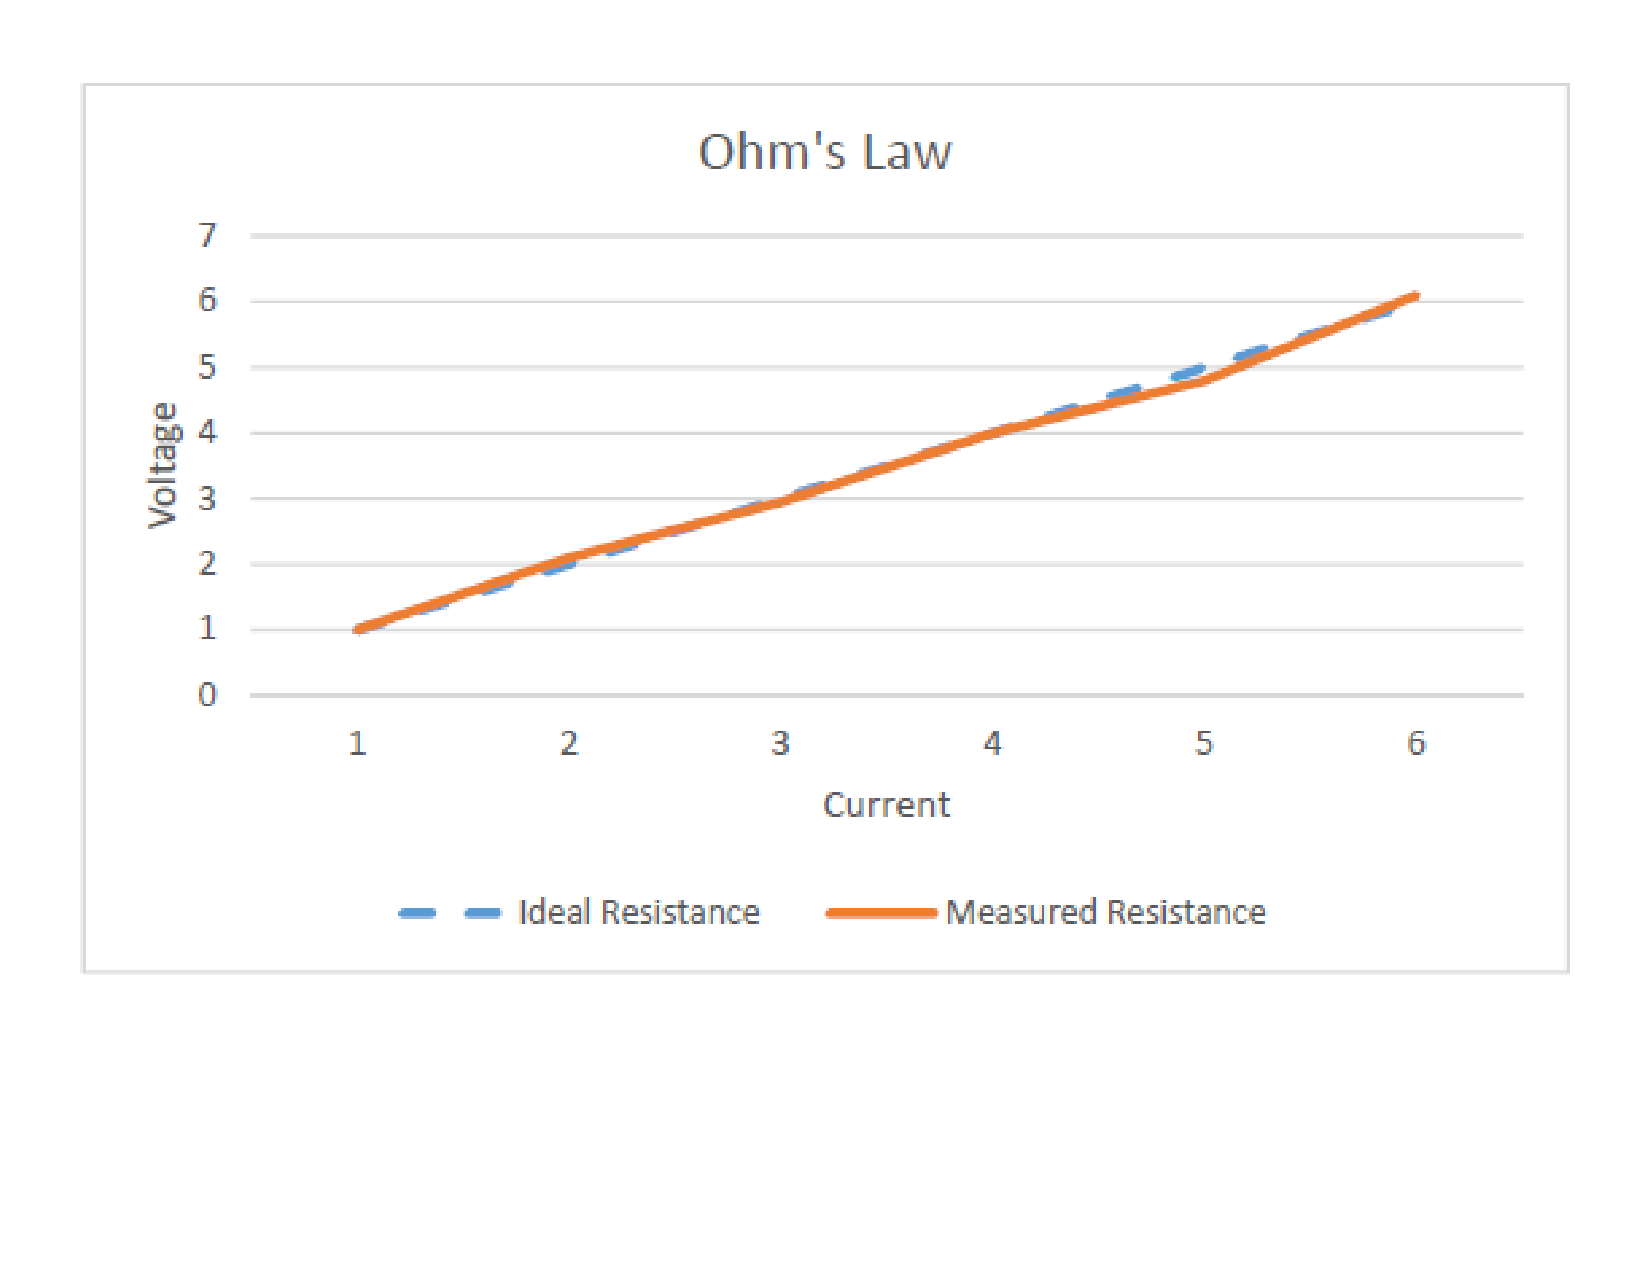
\includegraphics[width=0.7\linewidth]{./figure.pdf}
\caption{A Sample Graph}
\label{fig:figureforprinting}
\end{figure}
Current style is to place tables \emph{before} they are referenced with the caption above the table.  Figures are place \emph{after} they are referenced and the caption is below the figure.  If you have time, read the IEEE Style Sheet in the same folder with this sample.

Explain clearly what your results mean.  If you have a result that makes no sense, clearly state why it makes no sense.  If you can, give a plausible explanation as to what may have cause the strange result.  Do not try to hide a bad result.

\section{Conclusions}
Here you answer any questions raised in the previous sections.   You should end with a wrap--up and firm statement of what a great accomplishment this is.

% references section
%\baselineskip=.55\baselineskip

\bibliographystyle{IEEEtran}
\bibliography{references}

\newpage
\section*{Appendix}
An Appendix starts on a new page after everything else.  This is were your code will be.\\\\

\lstinputlisting{fragment.java}
\end{document}
